%%%%%%%%%%%%%%%%%%%%%%%%%%%%%%%%%%%%%%%%%
% 
% This template has been adapted by Thomas Höhener to fit the requirements for
% for a PhD-Thesis at the Graduate School for Cellular and Biomedical Sciences
% (GCB) of the University of Bern. 
%
% Check current guidlines on:
% https://www.gcb.unibe.ch/phd_program/phd_thesis_defense__degree/index_eng.html
%
% The template is based on: 
% Masters/Doctoral Thesis 
% LaTeX Template
% Version 2.5 (27/8/17)
%
% This template was downloaded from:
% http://www.LaTeXTemplates.com
%
% Version 2.x major modifications by:
% Vel (vel@latextemplates.com)
%
% This template is based on a template by:
% Steve Gunn (http://users.ecs.soton.ac.uk/srg/softwaretools/document/templates/)
% Sunil Patel (http://www.sunilpatel.co.uk/thesis-template/)
%
% Template license:
% CC BY-NC-SA 3.0 (http://creativecommons.org/licenses/by-nc-sa/3.0/)
%
%%%%%%%%%%%%%%%%%%%%%%%%%%%%%%%%%%%%%%%%%

%----------------------------------------------------------------------------------------
%	PACKAGES AND OTHER DOCUMENT CONFIGURATIONS
%----------------------------------------------------------------------------------------

\documentclass[
11pt, % The default document font size, options: 10pt, 11pt, 12pt
oneside, % Two side (alternating margins) for binding by default, uncomment to switch to one side
english, % ngerman for German
singlespacing, % Single line spacing, alternatives: onehalfspacing or doublespacing
%draft, % Uncomment to enable draft mode (no pictures, no links, overfull hboxes indicated)
%nolistspacing, % If the document is onehalfspacing or doublespacing, uncomment this to set spacing in lists to single
liststotoc, % Uncomment to add the list of figures/tables/etc to the table of contents
%toctotoc, % Uncomment to add the main table of contents to the table of contents
%parskip, % Uncomment to add space between paragraphs
%nohyperref, % Uncomment to not load the hyperref package
headsepline, % Uncomment to get a line under the header
chapterinoneline, % Uncomment to place the chapter title next to the number on one line
consistentlayout, % Uncomment to change the layout of the declaration, abstract and acknowledgements pages to match the default layout
]{MastersDoctoralThesis} % The class file specifying the document structure

\usepackage[utf8]{inputenc} % Required for inputting international characters
\usepackage[T1]{fontenc} % Output font encoding for international characters
\usepackage{subcaption}

\usepackage{mathpazo} % Use the Palatino font by default

\usepackage[backend=biber,style=numeric,natbib=true, sorting=none]{biblatex} % Use the bibtex backend with the authoryear citation style (which resembles APA)

\addbibresource{cdr.bib} % The filename of the bibliography

\usepackage[autostyle=true]{csquotes} % Required to generate language-dependent quotes in the bibliography

\usepackage{svg}
\usepackage[]{hyperref}
\usepackage[nameinlink]{cleveref} % Easy references to Figures, Tables and sections (\cref{})
\usepackage{pdfpages} % insert pdf documents
\usepackage[pagestyles]{titlesec} % remove the prefix ChapterN from the chapter name and in the headers
%\titleformat{\chapter}[display]{\normalfont\bfseries}{}{0pt}{\Huge}

\usepackage{makecell}
% \usepackage[section]{placeins}


\newpagestyle{mystyle}
{\sethead[\thepage][][\chaptertitle]{}{}{\thepage}}
\pagestyle{mystyle}
\setcounter{tocdepth}{1} % adjust depth of TOC: 0-chapter, 1-sectiom, 2-subsection

% no new page for the chapters
\usepackage{etoolbox}
\makeatletter
\patchcmd{\chapter}{\if@openright\cleardoublepage\else\clearpage\fi}{}{}{}
\makeatother

\usepackage{float}

%----------------------------------------------------------------------------------------
%	MARGIN SETTINGS
%----------------------------------------------------------------------------------------

\geometry{
	paper=a4paper, % Change to letterpaper for US letter
	outer=2.5cm, % Inner margin
	inner=2.5cm, % Outer margin  vorher 3.8
	bindingoffset=.5cm, % Binding offset
	top=1.5cm, % Top margin
	bottom=1.5cm, % Bottom margin
	% showframe, % Uncomment to show how the type block is set on the page
}

%----------------------------------------------------------------------------------------
%	THESIS INFORMATION
%----------------------------------------------------------------------------------------

% Those information will be used to generate the title page and the abstract. You can also access this information with the corresponding keyword. 

% Keywords used in the template. 
\thesistitle{JassBot
} % Your thesis title, print it with \ttitle
\supervisor{} % Your supervisor's name, print it with \supname. Include academic title.
\coadvisor{} %Your co-advisors's name, print it with \coaname. Include academic title.
\firstname{Raphael} % Your first name, print it with \fname. 
\lastname{Ziegler} % Your last name, print it with \lname .
\author{\fname~ \lname} % Your whole name made from your input, print it with \authorname.
\matriculationnumber{} % Your matriculation number, print it with \matrnumber
\degree{CAS in Applied Data Science} % Your degree name, print it with \degreename. 
%Possible degrees at the GCB: PhD in Biochemistry and Molecular Biology, PhD in Cell Biology, PhD in Biomedical Engineering, PhD in Biomedical Sciences, PhD in Immunology, PhD in Neuroscience, Doctor of Medicine and Philosophy (MD,PhD), Doctor of Veterinary Medicine and Philosophy (DVM,PhD), Doctor of Dentistry and Philosophy (DDS,PhD), PhD in Computational Biology, 
\institute{{}} % Your department's name and URL, print it with \instname
\faculty{{}} % Your department's name and URL, print it with \facname. Possible faculties: Faculty of Medicine, Faculty of Science, Vetsuisse Faculty, Institute of Virology and Immunology IVI, Mittelhäusern, Institute for Research in Biomedicine IRB, Bellinzona
\university{\href{https://www.unibe.ch/index_eng.html}{University of Bern}} % Your university's name and URL, print it with \univname. Possible Universities: University of Bern or University of Zurich (for Vetsuisse Zürich) 

% The following keywords are not used in this template. But define it if you want to use it in the text. 
%\department{{}} % Your department's name and URL, print it with \deptname
%\group{\href{https://www.GROUP_NAME.net/}{Group name}} % Your research group's name and URL, print it with \groupname
\subject{Project Report \\} % Your subject area, print it with \subjectname
\keywords{CAS, ADS, 2022} % Keywords for your thesis, print it with \keywordnames


%----------------------------------------------------------------------------------------
%	PDF META DATA
%----------------------------------------------------------------------------------------

\AtBeginDocument{
\hypersetup{pdftitle=\ttitle} % Set the PDF's title to your title
\hypersetup{pdfauthor=\authorname} % Set the PDF's author to your name
\hypersetup{pdfkeywords=\keywordnames} % Set the PDF's keywords to your keywords
}


%----------------------------------------------------------------------------------------
%	DOCUMENT STARTS
%----------------------------------------------------------------------------------------

\begin{document}

\frontmatter % Use roman page numbering style (i, ii, iii, iv...) for the pre-content pages

\pagestyle{plain} % Default to the plain heading style until the thesis style is called for the body content


%----------------------------------------------------------------------------------------
%	TITLE PAGE
%----------------------------------------------------------------------------------------
\begin{titlepage}
{
\vspace*{-3cm}
\hfill
\includesvg[scale= 0.7]{Extra/Logo_UniBe.svg} % University logo
}
 \begin{center}
\hypersetup{hidelinks} 
 \vspace*{.06\textheight}
  \vspace{3.0cm}
  {\Large Data Science Project}\\[1.0cm]
  {\Huge \bfseries \ttitle\par}\vspace{0.4cm} % Thesis title
  {\Huge \bfseries Project Report}\\[1.0cm] % graduate school name
  \Large June 15, 2023 \\[5.0cm]  % Datum 
  \vfill
  {\Large \authorname \\ 
   \href{mailto:raphael.ziegler@gmail.com}{raphael.ziegler@gmail.com} \par}\vspace{0.4cm} % Author name 

  % {\Large \degreename \par}


\end{center}
\end{titlepage}




%----------------------------------------------------------------------------------------
%	ABSTRACT PAGE
%----------------------------------------------------------------------------------------

\begin{abstract}
\addchaptertocentry{\abstractname} % Add the abstract to the table of contents

This project report presents the JassBot, a data science project focused on training an intelligent agent to play the Swiss card game Jass. The project aims to train a reinforcement learning algorithm to learn and implement an optimal game strategy. The project uses the two-player Handjass variant and excludes elements such as Marriage and Melds for simplicity. The report explores different reinforcement learning algorithms, including Monte Carlo Control, SARSA($ \lambda $), and Value Approximation. The game environment, agents, actions, and various card encoding methods are described. The report concludes by analyzing the results obtained from different encoding approaches. \\

While macro patterns are observed, no apparent, detailed patterns emerge. The findings indicate the potential for using reinforcement learning in developing game strategies and suggest avenues for future enhancements to the JassBot project.



\end{abstract}
\newpage

%----------------------------------------------------------------------------------------
%	LIST OF CONTENTS/FIGURES/TABLES PAGES
%----------------------------------------------------------------------------------------

{
  \hypersetup{linkcolor=black} % Make links black in table of content  
  \tableofcontents % Prints the main table of contents
  \newpage
}



%----------------------------------------------------------------------------------------
%	THESIS CONTENT - CHAPTERS
%----------------------------------------------------------------------------------------

\mainmatter % Begin numeric (1,2,3...) page numbering

\pagestyle{Rzi} % Return the page headers back to the "thesis" style

% Include the chapters of the thesis as separate files from the Chapters folder
% Uncomment the lines as you write the chapters


% Chapter Template

\chapter{Project Objectives} % Main chapter title

\label{Chapter1} % Change X to a consecutive number; for referencing this chapter elsewhere, use \cref{ChapterX}

%----------------------------------------------------------------------------------------
%	SECTION 1
%----------------------------------------------------------------------------------------


For this project, a JassBot is created and trained to play against itself.
For this purpose, a reinforcement learning algorithm will be trained to find the best game strategy.
The baseline will be the random pick of a playable card for comparison.\\

\section{Deck \cite{jass}}
Jass is played with a deck of 36 cards (Ace, King, Queen, Jack, 10, 9, 8, 7, 6) Swiss-French or Swiss-German cards (Ass, König, Ober, Under, Banner (= 10), 9, 8, 7, 6). The Swiss-German cards use Swiss suits, a variant of German suits, and have a distinctive design.\\


The game is traditionally played with Swiss-suited cards east of the Brünig-Napf-Reuss line \cite{reuss} and with French cards in western Switzerland. \\
The Swiss suits are Rosen (roses), Eicheln (acorns), Schellen (bells), and Schilten (shields)
\begin{figure}[ht!]
    \centering
    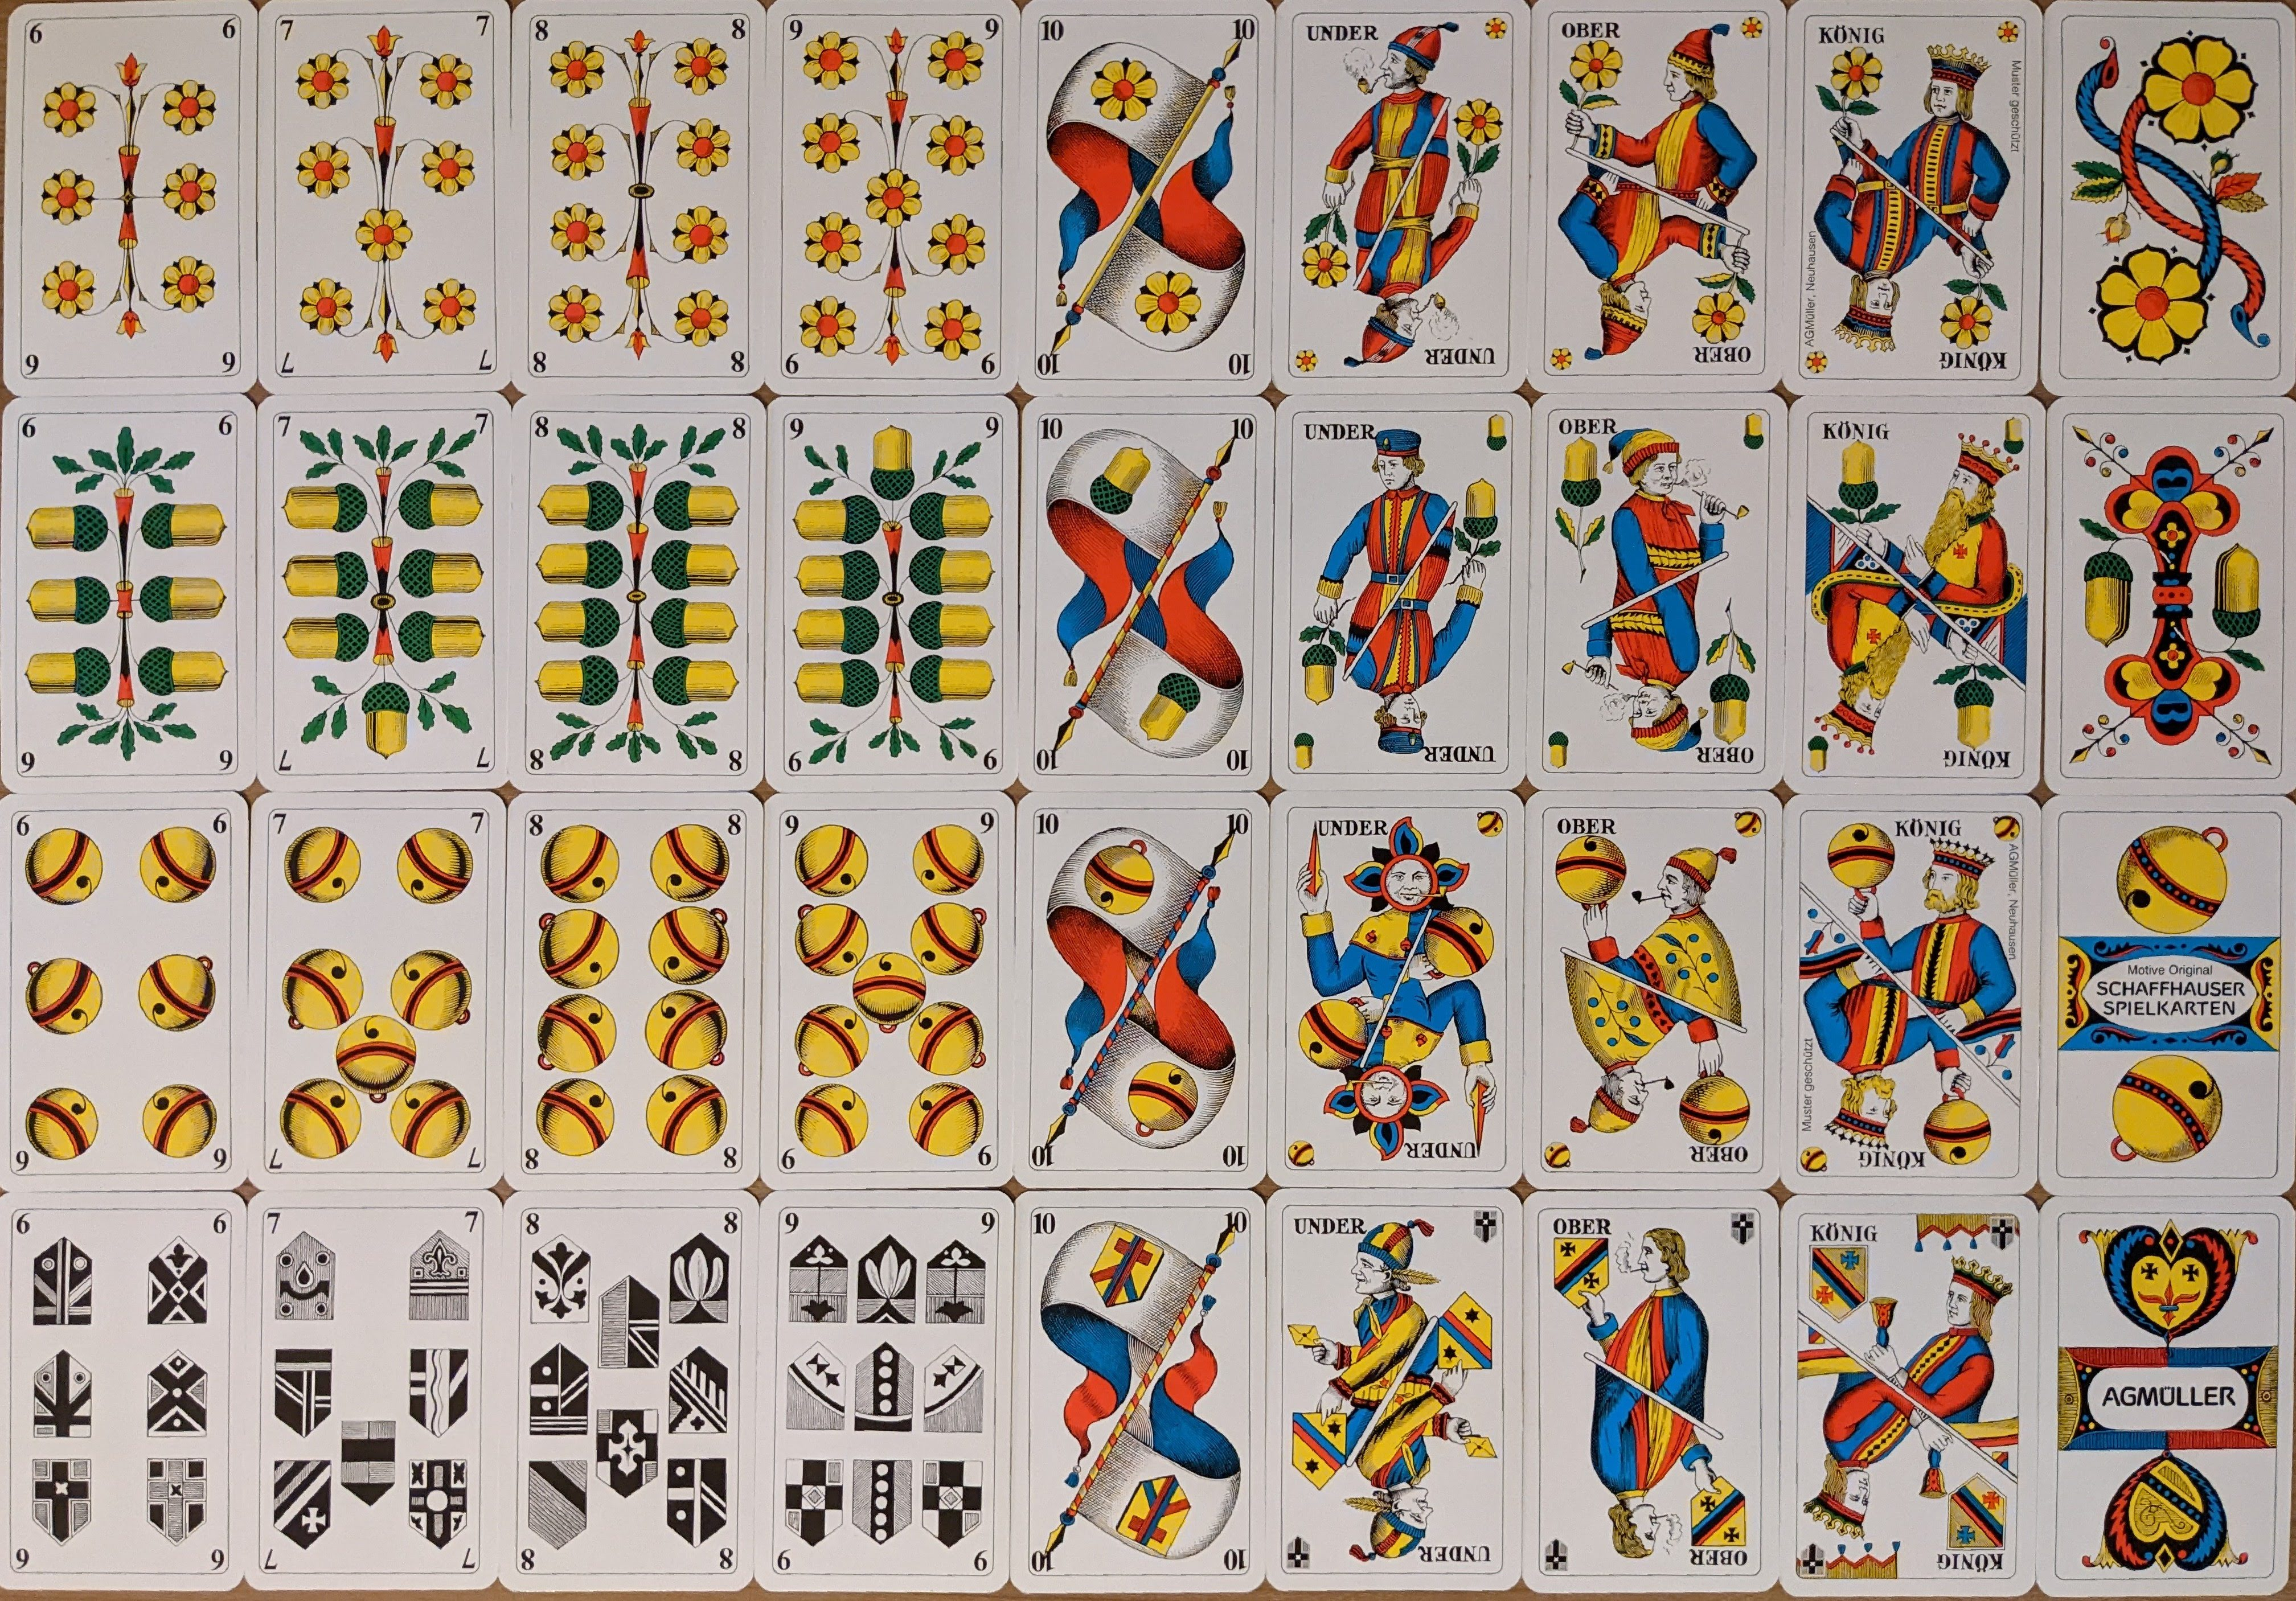
\includegraphics[width=1.0\textwidth]{Figures/jasskarten_de_ch}
    \decoRule
    \caption[Swiss German Cards]{Swiss German Cards}
    \label{fig:SwissGermanCards}
\end{figure}



\section{Game variants}
Jassen is the collective term for different game variants with different numbers of players. In most variants, each player receives nine cards (hand).
The most popular variant is the Schieber, where two teams of 2 players play against each other until one team reaches the points needed to win.
Another well-known game variant is the Differenzler (known from the TV show Samstagsjass). Here four players play against each other; before each deal, each player announces how many points he intends to make in this round. The difference to the actual score is noted as penalty points and added at each round. The player with the least penalty points wins.
Another game variant is the Handjass, which can be played in pairs, threes, or fours. In each round, the player who takes the most points scores a stroke, and anyone who takes fewer than 26 points gets a Null - sometimes known as a Herdöpfel (potato) - which is worth minus one stroke. The player who achieves a net score of 7 strokes wins and retires from the game: the loser is the last player who fails to reach seven strokes. \cite{handjass}\\

\section{Rules \cite{jass}}
Jass is a game of points scored for three features: Stöck, Wiis, and Stich, respectively, "marriages, melds, tricks.


\subsection{Tricks}

The trump Jack, also called Puur, counts 20 and is the highest card in the game. The trump Nine, or Nell, Näll, is the second-best card. Plain suit numerals below 10 count nothing. The total value of all counters in the pack is 152, that is, 62 in trumps plus 30 in each plain suit. Winning the last trick scores an additional 5 points. Hence the total possible for the third scoring feature, "tricks," usually is 157 points.

The rank of the cards, from highest to lowest, and their values in card points are shown in the following table:

\begin{table}[ht!]
    \caption{Card Values - trump games}
    \label{tab:Card Values - trump games}
    \begin{center}
        \begin{tabular}{|l|c|c|c|c|c|c|c|c|c|c|c|}
             \hline
             \multicolumn{12}{|c|}{\textbf{Card Values}} \\ \hline
             Plain suit rank & & & A & K & O/Q & U/J & 10 & 9 & 8 & 7 & 6 \\ \hline
             Value & 20 &  14 & 11 & 4 & 3 &   & 10 &   & 0 & 0 & 0 \\ \hline
             Trump suit rank & J/U & 9 & A & K & O/Q & U/J & 10 & 9 & 8 & 7 & 6 \\ \hline
        \end{tabular}
    \end{center}
\end{table}

The no-trumps game called Obenabe and Undenufe, in which the ranks are reversed, are shown in the following table:
\begin{table}[ht!]
    \caption{Card Values - no-trump games}
    \label{tab:Card Values - no-trump games}
    \begin{center}
        \begin{tabular}{|l|c|c|c|c|c|c|c|c|c||c|c|c|c|c|c|c|c|c|}
             \hline
             \multicolumn{19}{|c|}{\textbf{Card Values}} \\ \hline
             \multicolumn{10}{|c||}{Obenabe} & \multicolumn{9}{c|}{Undenufe} \\ \hline
             Rank & A & K & O/Q & U/J & 10 & 9 & 8 & 7 & 6 & 6 & 7 & 8 & 9 & 10 & U/J & O/Q & K & A  \\ \hline
             Value & 11 & 4 & 3 & 2 & 10 & 0 & 8 & 0 & 0 & 11 & 0 & 8 & 0 & 10 & 2 & 3 & 4 & 0 \\ \hline
        \end{tabular}
    \end{center}
\end{table}


\subsection{Marriage}
Marriage (Stöck): A marriage is the holding in one hand of the König and Ober (King and Queen) of trump. Its holder claims it upon the second of them to a trick. Its score of 20 is recorded as if made before those for melds and tricks, even though it is not revealed until after melds have been declared.

\subsection{Melds}
Meld (Wys or Weis): A meld is a suit sequence of three or more cards or a quartet of Aces, Kings, Queens, or Jacks scoring as follows:
    
\begin{itemize}
    \item Four Jacks: scores 200
    \item Four 9's: scores 150
    \item Five or more in suit sequence: scores 100
    \item Four A, K, Q, 10: scores 100
    \item Four in suit sequence: scores 50
    \item Three in suit sequence: scores 20
\end{itemize} 
        
A card may not be used in two melds at once, though the trump King or Queen may belong to a meld in addition to being married; that is, a player holding four Kings and a sequence of four to the Ace or King would count only 100 for Kings, not also 50 for the sequence.



\section{Chosen Game and Rules for this Project}
For this project, a two-player Handjass was used, hoping to minimize the game's complexity. It was also decided not to use Marriage and Melds, as these scores are obtained randomly and do not contribute to learning a game strategy. A further decision was not to implement the five scores for the last-round winner to minimize the programming effort.
If this project finds a successful game strategy, the remaining game elements can be added in a later version.\\






 
\newpage
\input{Chapters/Chapter2_Descriptive_Statistics} 
\input{Chapters/Chapter3_Machine_Learning}
% Chapter Template

\chapter{Results} % Main chapter title

\label{Chapter4} % Change X to a consecutive number; for referencing this chapter elsewhere, use \cref{ChapterX}

%----------------------------------------------------------------------------------------
%	SECTION 1
%----------------------------------------------------------------------------------------
The results of the different card encodings (MCC Figure \ref{fig:Monte Carlo Control: Q value function with different card encodings} and SARSA Figure \ref{fig:SARSAl: Q value function with different card encodings}) show patterns in the macro range, but no clear pattern can be seen in detail. The macro pattern is explained by the fact that certain card combinations cannot occur and therefore have zero value. As expected, the different card encodings produce different patterns. \\

% \section{Monte Carlo Controll (MCC}
% \newpage

\begin{figure}[ht!]
    \begin{subfigure}{0.5\textwidth}
        \includegraphics[width=1\linewidth]{Figures/mcc_simple_10000000_random} 
        \caption[Simple]{Simple}
        \label{fig:mccSimple}
    \end{subfigure}
    \begin{subfigure}{0.5\textwidth}
        \includegraphics[width=1\linewidth]{Figures/mcc_linear_numbering_10000000_random}
        \caption[Linear Numbering]{Linear Numbering}
        \label{fig:mcclinear numbering}
    \end{subfigure} \\
    \begin{subfigure}{0.5\textwidth}
        \includegraphics[width=1\linewidth]{Figures/mcc_card_strength_10000000_random}
        \caption[Card Strength]{Card Strength}
        \label{fig:mcccard strength}
    \end{subfigure}
    \begin{subfigure}{0.5\textwidth}
        \includegraphics[width=1\linewidth]{Figures/mcc_digits1_10000000_random} 
        \caption[Digits1]{Digits1}
        \label{fig:mccdigits1}
    \end{subfigure} \\
    \begin{subfigure}{0.5\textwidth}
        \includegraphics[width=1\linewidth]{Figures/mcc_digits2_10000000_random}
        \caption[Digits2]{Digits2}
        \label{fig:mccdigits2}
    \end{subfigure}
    \caption{Monte Carlo Control: Q value function with different card encodings}
\label{fig:Monte Carlo Control: Q value function with different card encodings}
\end{figure}



% \section{SARSA($ \lambda $)}
% \newpage

\begin{figure}[ht!]
    \begin{subfigure}{0.5\textwidth}
        \includegraphics[width=1\linewidth]{Figures/SARSA_simple_1000000_random} 
        \caption[Simple]{Simple}
        \label{fig:SARSASimple}
    \end{subfigure}
    \begin{subfigure}{0.5\textwidth}
        \includegraphics[width=1\linewidth]{Figures/SARSA_linear_numbering_1000000_random}
        \caption[Linear Numbering]{Linear Numbering}
        \label{fig:SARSAlinear numbering}
    \end{subfigure} \\
    \begin{subfigure}{0.5\textwidth}
        \includegraphics[width=1\linewidth]{Figures/SARSA_card_strength_1000000_random}
        \caption[Card Strength]{Card Strength}
        \label{fig:SARSAcard strength}
    \end{subfigure}
    \begin{subfigure}{0.5\textwidth}
        \includegraphics[width=1\linewidth]{Figures/SARSA_digits1_1000000_random} 
        \caption[Digits1]{Digits1}
        \label{fig:SARSAdigits1}
    \end{subfigure} \\
    \begin{subfigure}{0.5\textwidth}
        \includegraphics[width=1\linewidth]{Figures/SARSA_digits2_1000000_random}
        \caption[Digits2]{Digits2}
        \label{fig:SARSAdigits2}
    \end{subfigure}
    \caption{SARSA: Q value function with different card encodings}
\label{fig:SARSAl: Q value function with different card encodings}
\end{figure}



\newpage


The two RL algorithms require vastly different execution times. MCC can execute more episodes in less time than SARSA. For the MCC plots, 10 million episodes were used; this was not practical for SARSA since it requires many times more computation time, and the card encoding affects the computation times. \\

The two RL algorithms reveal similar patterns; MCC shows a more uniform Q value function due to the larger number of episodes. However, it can be seen that the SARSA algorithm shows a similar tendency. See Appendix \ref{MCC and SARSA plots side by side with the same card coding} MCC and SARSA plots side by side with the same card encoding. \\

The development of the Q value function in dependence on the different numbers of episodes is shown in Figure \ref{fig:Monte Carlo Control: Evolution of Q value function with more episodes}. The greater the number of episodes, the more apparent the pattern. At 100 million episodes, a clear pattern can be seen. \\

\begin{figure}[ht!]
    \begin{subfigure}{0.5\textwidth}
        \includegraphics[width=1\linewidth]{Figures/mcc_card_strength_1000000_random} 
        \caption[Card Strength with 1'\,000'\,000 episodes]{Card Strength with 1'\,000'\,000 episodes}
        \label{fig:mcc1}
    \end{subfigure}
    \begin{subfigure}{0.5\textwidth}
        \includegraphics[width=1\linewidth]{Figures/mcc_card_strength_10000000_random}
        \caption[Card Strength with 10'\,000'\,000 episodes]{Card Strength with 10'\,000'\,000 episodes}
        \label{fig:mcc10}
    \end{subfigure} \\
    \begin{subfigure}{0.5\textwidth}
        \includegraphics[width=1\linewidth]{Figures/mcc_card_strength_100000000_random}
        \caption[Card Strength with 100'\,000'\,000 episodes]{Card Strength with 100'\,000'\,000 episodes}
        \label{fig:mcc100}
    \end{subfigure}
\caption{Monte Carlo Control: Evolution of Q value function with more episodes}
\label{fig:Monte Carlo Control: Evolution of Q value function with more episodes}
\end{figure}


A comparison with a Q value function where the agent can only randomly select a card shows the same pattern (\ref{fig:Comparison: MCC with different decision options}), confirming that the RL can not demonstrate learning success. This result confirms the "independent" test performed on a second game engine (Jupyter Notebook: dashboard.ipynb, see Github \cite{code}). The test lets two agents play against each other; AGENT 1 uses the learned Q-value function, and AGENT 2 randomly chooses a card. After a million games, AGENT 1 (Q value function) is in the lead with 51\%.


  
\begin{figure}[ht!]
    \begin{subfigure}{0.5\textwidth}
        \includegraphics[width=1\linewidth]{Figures/mcc_simple_10000000_random} 
        \caption[RL with options take or leave]{RL with options take or leave}
        \label{fig:RL with options take or leave}
    \end{subfigure}
    \begin{subfigure}{0.5\textwidth}
        \includegraphics[width=1\linewidth]{Figures/mcc_simple_10000000_random_2}
        \caption[RL with option random]{RL with option random}
        \label{fig:RL with option random}
    \end{subfigure} \\
    \caption{Comparison: MCC with different decision options}
\label{fig:Comparison: MCC with different decision options}
\end{figure}


% Chapter Template

\chapter{Conclusion} % Main chapter title

\label{Chapter6} % Change X to a consecutive number; for referencing this chapter elsewhere, use \cref{ChapterX}

%----------------------------------------------------------------------------------------
%	SECTION 1
%----------------------------------------------------------------------------------------

The two ML algorithms (MCC, SARSA) could not achieve any  meaningful learning success, or more precisely, the learned Q value function does only achive a 1\% better result than a randomly played card. \\

The fact that not all possible hand variations were played through could also have contributed to the poor performance. The RL needed more opportunities to learn all the variants. \\

\noindent
The considerations to encode the game states were not fully successful.

\begin{itemize}
    \item One possible reason is that "only" two actions are available (take, leave). However, it cannot be guaranteed that the action can be executed (e.g., a take action cannot have a card in hand to take the trick).
    \item The changing of the dealer (the winner of the last round plays the first card in the current round) leads to the fact that the actions do not reflect the actual state of the game because the player who deals can only partially judge whether an action (take/leave) is possible.
    \item If the desired action was impossible, a playable card was randomly selected. This should have been considered a learning termination (terminal).
\end{itemize} 


\noindent
The example of Easy 21 was not transversally for Jass, which allows more game states. It should be possible to consider more than two game state:
\begin{itemize}
    \item Consideration of trump suit
    \item Who plays the first card in a round (for the first and second players, there are two different strategies to learn).
    \item Does the player have the cards to decide if he can take or leave? Only if both possibilities exist can something be learned about the game strategy (take/leave).
\end{itemize}

\vspace*{0.5cm}

\noindent
The example shown in Figure \ref{fig:mcc100} with 100 million episodes suggests that we have been working with too few episodes. The illustrated case with the card encoding card strength is unsuitable with the current environment for the independent test since as several cards, can have the same value. \\
If the project is pursued further, either optimization must be found in the current Python code to speed up the execution time or more powerful hardware is needed. 


\newpage

%----------------------------------------------------------------------------------------
%	ACKNOWLEDGEMENTS
%----------------------------------------------------------------------------------------

\begin{acknowledgements}
\addchaptertocentry{\acknowledgementname} % Add the acknowledgements to the table of contents
%The acknowledgments and the people to thank go here, don't forget to include your project advisor\ldots

I thank everyone who accompanied me during the CAS Applied Data Science.  \\

\noindent
Special thanks go to Sigve Haug and Mykhailo Vladymyrov, with whom we often had exciting conversations about all and everything and, of course, also in professional matters. \\

\noindent
Furthermore, I would like to thank all the other lecturers/referees who always actively supported us and patiently answered our questions. \\

\noindent
Another thank goes to my fellow students; seeing and exchanging ideas with them was always delightful. \\

\noindent
Last but not least, I would like to thank Matyas Amrouche for writing the article \textit{"Playing Cards with Reinforcement Learning"} \cite{easy21} and providing the JupyterNotebook \cite{easy21_explanation}.


\end{acknowledgements}
\newpage




%----------------------------------------------------------------------------------------
%	THESIS CONTENT - APPENDICES
%----------------------------------------------------------------------------------------

\appendix % Cue to tell LaTeX that the following "chapters" are Appendices

% Include the appendices of the thesis as separate files from the Appendices folder
% Uncomment the lines as you write the Appendices

% Chapter Template

\chapter{Github Repository} % Main chapter title

\label{Github Repository} % Change X to a consecutive number; for referencing this chapter elsewhere, use \cref{ChapterX}


Mentioning of essential files: \\

\noindent
\textbf{{\LARGE python}} \\

\noindent
For running the code, the minimum required Python version is 3.10 \\

\noindent
\textbf{Easy 21}
\begin{itemize}
    \item Easy 21 Jupyter Notebook
\end{itemize}

\noindent
\textbf{jassbot}  
\begin{itemize}
    \item config.py: Configure everything in this file (different card encodings), and for ease of use, start the RL and plot the Q value function.
    \item env.py: Jass environment for interaction with the RL algorithms
    \item ai\_functionality.py: logic for deciding what card to play
    \item function.py: functions for card encoding
    \item plotting.py: functionality for the different plots
    \item monte\_carlo\_control.py: Monte Carlo Control functionality
    \item sarsa.py: SARSA functionality
    \item dashbord.ipynd: Jupyter Notebook to determine if we learned something (testing) - configuration made in the config.py file
    \item game\_engine.py: Jass game-engine (environment) for the testing
\end{itemize}

\noindent
\textbf{Easy 21}
\begin{itemize}
    \item \LaTeX\ source files
\end{itemize}

\include{Appendices/AppendixB}


%----------------------------------------------------------------------------------------
%	BIBLIOGRAPHY
%----------------------------------------------------------------------------------------


\renewcommand{\bibname}{Reference}
\printbibliography[heading=bibintoc]
\newpage


%-----------------------------------------------------------------------------------------
%   Liste der Figuren und Tabellen
%-----------------------------------------------------------------------------------------

{
\hypersetup{linkcolor=black} % Make links black in table of content 
\listoffigures % Prints the list of figures
\listoftables % Prints the list of tables
}

%----------------------------------------------------------------------------------------
%	ABBREVIATIONS
%----------------------------------------------------------------------------------------

\begin{abbreviations}{ll} % Include a list of abbreviations (a table of two columns)
\textbf{ML} & Machine Learning\\
\textbf{RL} & Reinforcement Learning\\
\textbf{MCC} & Monte Carlo Control\\
\textbf{SARSA} & State, Action, Revard, State', Action'  \hspace*{6cm}\\
\textbf{VA} & Value Approximation


\end{abbreviations}
\newpage


\cleardoublepage


\end{document}  
